\documentclass[11pt]{article}

\usepackage[margin=1in]{geometry}
\usepackage{amsmath,amssymb,mathtools}
\usepackage{booktabs}
\usepackage{graphicx}
\usepackage{float}

\setlength{\parindent}{0pt}
\setlength{\parskip}{0.55em}
\renewcommand{\arraystretch}{1.15}

\newcommand{\sech}{\operatorname{sech}}
\newcommand{\norm}[1]{\left\lVert #1\right\rVert}

\title{Problem 4 Handout I\\Travelling-Wave Solution of Viscous Burgers' Equation}
\author{Rishabh Kumar}
\date{\today}

\begin{document}
\maketitle

\section{Problem}

The viscous Burgers' equation is
\begin{equation}
    u_t+u u_x=\varepsilon u_{xx},
    \qquad x\in\mathbb{R},\quad t>0,\quad \varepsilon>0.
    \label{eq:burgers}
\end{equation}
The assignment asks us to show that
\begin{equation}
    u(x,t)=
    \omega\left(1-\tanh\left[
    \frac{\omega}{2\varepsilon}(x-\omega t-x_0)
    \right]\right)
    \label{eq:tw}
\end{equation}
is an exact travelling-wave solution.  Here $\omega$ is a constant wave speed and
$x_0$ is the centre of the transition layer.

\section{Travelling-Wave Ansatz}

Introduce the travelling coordinate
\begin{equation}
    y=x-\omega t-x_0,
    \qquad
    u(x,t)=w(y).
\end{equation}
Then
\begin{equation}
    u_t=-\omega w',
    \qquad
    u_x=w',
    \qquad
    u_{xx}=w''.
\end{equation}
Substitution into \eqref{eq:burgers} gives the ordinary differential equation
\begin{equation}
    -\omega w'+w w'=\varepsilon w''.
\end{equation}
Since $w w'=(w^2/2)'$, this may be written as
\begin{equation}
    -\omega w'+\left(\frac{w^2}{2}\right)'=\varepsilon w''.
\end{equation}

\section{First Integral}

Integrating once with respect to $y$ gives
\begin{equation}
    -\omega w+\frac{w^2}{2}=\varepsilon w' + C.
    \label{eq:first-integral}
\end{equation}
For the shock-like front in the problem,
\begin{equation}
    w(-\infty)=2\omega,
    \qquad
    w(+\infty)=0,
    \qquad
    w'(\pm\infty)=0.
\end{equation}
Evaluating \eqref{eq:first-integral} at $+\infty$ gives $C=0$.  Evaluating at
$-\infty$ is then automatically consistent, because
\begin{equation}
    -\omega(2\omega)+\frac{(2\omega)^2}{2}=0.
\end{equation}
Thus the first-order ODE is
\begin{equation}
    \varepsilon w'
    =
    -\omega w+\frac{w^2}{2}
    =
    \frac{w(w-2\omega)}{2}.
    \label{eq:separable-ode}
\end{equation}

\section{Solving the Separable ODE}

Equation \eqref{eq:separable-ode} is separable:
\begin{equation}
    \frac{dw}{w(w-2\omega)}
    =
    \frac{dy}{2\varepsilon}.
\end{equation}
Use the partial fraction identity
\begin{equation}
    \frac{1}{w(w-2\omega)}
    =
    \frac{1}{2\omega}
    \left(
    \frac{1}{w-2\omega}-\frac{1}{w}
    \right).
\end{equation}
Therefore
\begin{equation}
    \frac{1}{2\omega}
    \ln\left|\frac{w-2\omega}{w}\right|
    =
    \frac{y}{2\varepsilon}+C_1.
\end{equation}
The integration constant represents a horizontal shift of the wave and is absorbed
into $x_0$.  Since the desired front satisfies $0<w<2\omega$, it is convenient to
write the result as
\begin{equation}
    \frac{2\omega-w}{w}
    =
    \exp\left(\frac{\omega y}{\varepsilon}\right).
\end{equation}
Solving for $w$,
\begin{equation}
    w(y)
    =
    \frac{2\omega}{1+\exp(\omega y/\varepsilon)}.
    \label{eq:logistic}
\end{equation}
Finally, using
\begin{equation}
    \frac{2}{1+e^A}=1-\tanh\left(\frac{A}{2}\right),
\end{equation}
with $A=\omega y/\varepsilon$, \eqref{eq:logistic} becomes
\begin{equation}
    w(y)=
    \omega\left(1-\tanh\left(\frac{\omega y}{2\varepsilon}\right)\right).
\end{equation}
Substituting $y=x-\omega t-x_0$ gives exactly \eqref{eq:tw}.

\section{Direct Verification}

For an independent check, define
\begin{equation}
    \eta=\frac{\omega}{2\varepsilon}(x-\omega t-x_0),
    \qquad
    u=\omega(1-\tanh\eta).
\end{equation}
Then
\begin{equation}
    \eta_x=\frac{\omega}{2\varepsilon},
    \qquad
    \eta_t=-\frac{\omega^2}{2\varepsilon}.
\end{equation}
Using $(\tanh\eta)'=\sech^2\eta$ and
$(\sech^2\eta)'=-2\sech^2\eta\tanh\eta$, we obtain
\begin{align}
    u_x
    &=
    -\omega\sech^2\eta\,\eta_x
    =
    -\frac{\omega^2}{2\varepsilon}\sech^2\eta,
    \\
    u_t
    &=
    -\omega\sech^2\eta\,\eta_t
    =
    \frac{\omega^3}{2\varepsilon}\sech^2\eta,
    \\
    u_{xx}
    &=
    -\frac{\omega^2}{2\varepsilon}
    \left(-2\sech^2\eta\tanh\eta\right)\eta_x
    =
    \frac{\omega^3}{2\varepsilon^2}
    \sech^2\eta\,\tanh\eta.
\end{align}
Therefore
\begin{align}
    u_t+u u_x
    &=
    \frac{\omega^3}{2\varepsilon}\sech^2\eta
    -
    \frac{\omega^3}{2\varepsilon}(1-\tanh\eta)\sech^2\eta
    \\
    &=
    \frac{\omega^3}{2\varepsilon}
    \sech^2\eta\,\tanh\eta
    =
    \varepsilon u_{xx}.
\end{align}
Thus \eqref{eq:tw} satisfies Burgers' equation exactly.

\section{Interpretation}

The wave connects two constant states:
\begin{equation}
    \lim_{x\to-\infty}u(x,t)=2\omega,
    \qquad
    \lim_{x\to+\infty}u(x,t)=0.
\end{equation}
The centre of the transition layer is located at
\begin{equation}
    x=\omega t+x_0,
\end{equation}
so the front travels to the right with speed $\omega$.  The layer width is
proportional to $\varepsilon/\omega$.  As $\varepsilon$ decreases, the transition
becomes sharper and approaches an inviscid shock profile.

\section{Numerical Verification Figure}

In the notebook verification, the travelling wave is tested with
\begin{equation}
    \omega=0.5,
    \qquad
    \varepsilon=0.1,
    \qquad
    x_0=3,
    \qquad
    -5\le x\le 5,
    \qquad
    T=2.
\end{equation}
With $h=k=10^{-3}$, the reported maximum error is
\begin{equation}
    \norm{e(T)}_\infty=4.548\times10^{-7}.
\end{equation}

\begin{figure}[H]
    \centering
    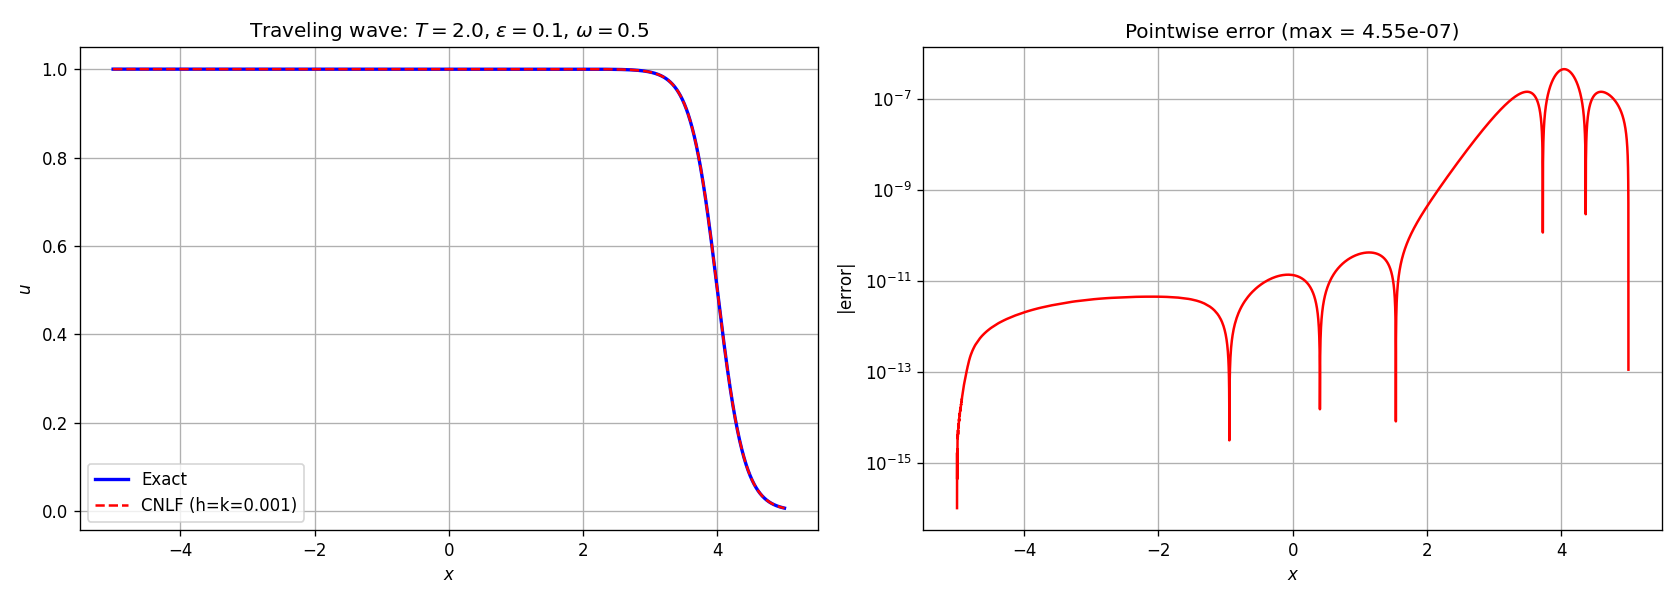
\includegraphics[width=\textwidth]{figures/traveling_wave.png}
    \caption{CNLF approximation of the travelling wave and pointwise error at $T=2$.}
\end{figure}

\end{document}
